\documentclass[a4paper,12pt]{article}
\usepackage{amssymb}
\usepackage{amsfonts}

% Кодировка и язык
\usepackage[utf8]{inputenc}
\usepackage[T2A]{fontenc}
\usepackage[russian]{babel}


% Математические пакеты
\usepackage{amsmath,amsfonts,amssymb}
%Таблицы
\usepackage{array}
\usepackage{booktabs} % Для более красивых горизонтальных линий в таблицах
\usepackage{graphicx}
\usepackage{array}
\usepackage{booktabs}
% Геометрия страницы
\usepackage{geometry}
\geometry{top=2cm, bottom=2cm, left=2.5cm, right=2.5cm}
% Гиперссылки (лучше загружать последним)
\usepackage{hyperref}


% Настройки заголовка
\title{Домашнее задание}
\author{Студент: \textbf{Ростислав Лохов}}
\date{\today}

\begin{document}

% Титульный лист
\begin{titlepage}
    \centering
    \vspace*{1cm}

    \Huge
    \textbf{Домашнее задание}

    \vspace{0.5cm}
    \LARGE
    По курсу: \textbf{Экономика}

    \vspace{1.5cm}

    \textbf{Студент: Ростислав Лохов}

    \vfill

    \Large
    АНО ВО Центральный университет\\
    \vspace{0.3cm}
    \today

\end{titlepage}

% Содержание
\tableofcontents
\newpage

% Основной текст
\section{Сине-Красный уровень}


\subsection{Задача 1}

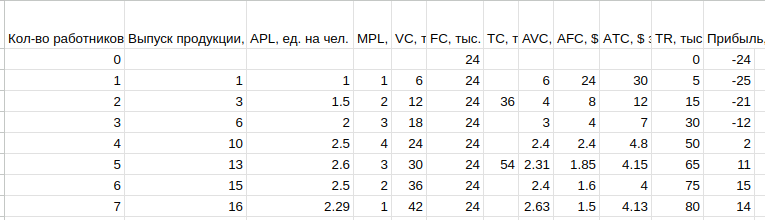
\includegraphics[scale=0.4]{graphs/5.1.png}

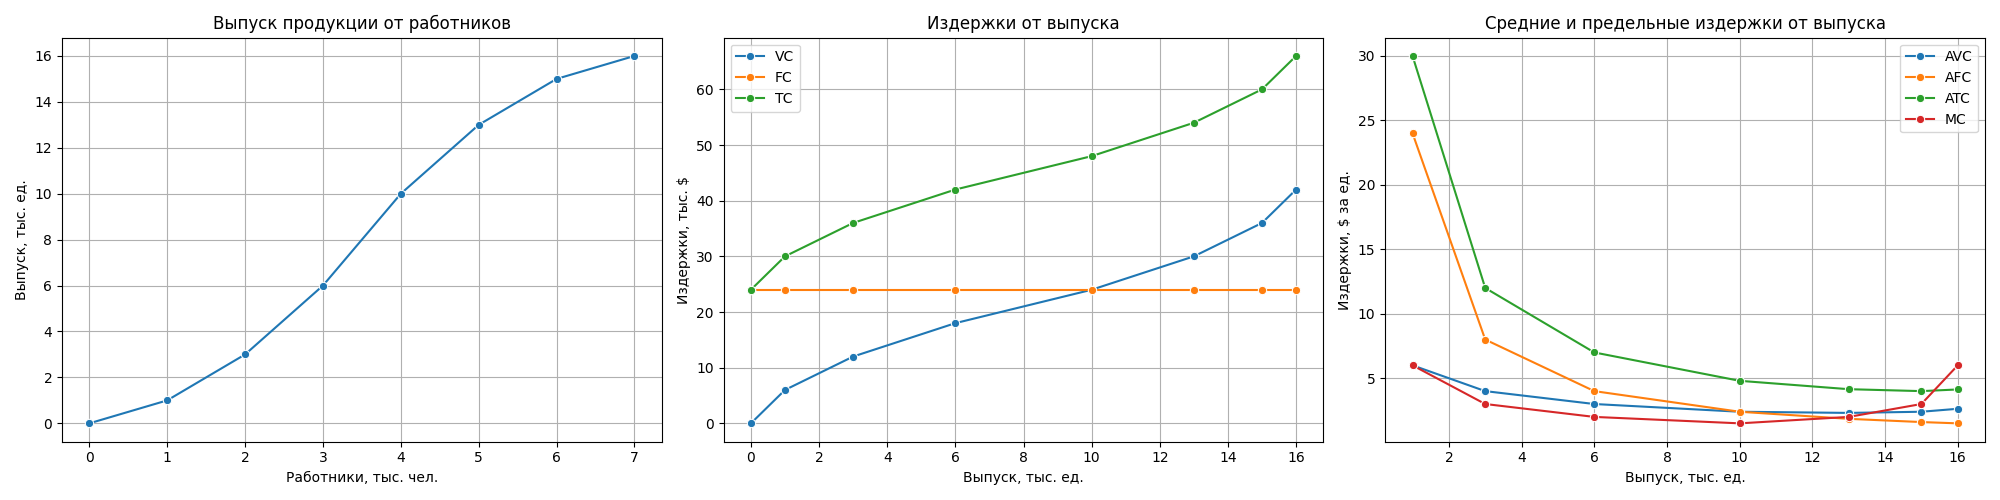
\includegraphics[scale=0.3]{graphs/5.2.png}


\subsection{Задача 2}
\begin{enumerate}
    \item Огромные затраты на разработку геннотерапевтического препарата
    \item Маленькая целевая аудитория 
\end{enumerate}

\subsection{Задача 3}
\begin{enumerate}
    \item $FC=1000$
    \item $VC = Q^3-10Q^2+300Q$
    \item $ATC = Q^2-10^Q+300+1000/Q$
    \item $AVC = Q^2-10Q+300$
    \item $AFC=1000/Q$
\end{enumerate}

\subsection{Задача 4}

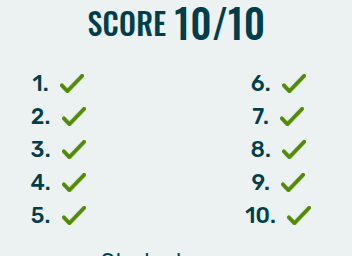
\includegraphics[scale=0.3]{graphs/5.3.png}

\subsection{Задача 5}
\begin{enumerate}
    \item ATC=100
    \item VC=300
\end{enumerate}

\subsection{Задача 6}
\begin{enumerate}
    \item Отсутствие рыночных стимулов, нет интереса напрямую предприятию увеличивать производство
    \item Бюрократия
    \item Неэффективное планирование могло привести к тому, что станки были не нужны
\end{enumerate}

\section{Черный уровень}

\subsection{Задача 1}
\begin{enumerate}
    \item Снижение издержек на закупку комплектующих
    \item Единый производственный процесс
    \item Сокращение времнеи на разработку клавиатуры
\end{enumerate}

\subsection{Задача 2}
\begin{enumerate}
    \item FC = Аренда капитала * количество капитала = 20 млн р в месяц
    \item $Q=TP = 10\sqrt{L} \Leftrightarrow L = \frac{Q^2}{100}$
    \item $VC = wL = 80000\cdot L \Rightarrow VC=800Q^2$ рублей
    \item $ATC(Q)=\frac{20000}{Q}+0.8Q$
\end{enumerate}

\subsection{Задача 3}
\begin{enumerate}
    \item Мясо птицы
    \item Снижение издержек сырья и материалов поставщиков на 6.62 (оптимизация использования сырья или переход на более дешевые материалы или поставщиков)
    \item Рост производственных расходов на 1.78 (увеличение затрат на энергоносители, инвестиции в модернизацию оборудования)
    \item Снижение налоговой нагрузки на 4.21 (льготы или перераспределение между этими цепочками)
    \item Снижение трат на логистику на 1.5 (оптимизация логических маршрутов за счет цифровизации)
    \item Увеличение прибыли на 1 (увеличение обьемов и оптимизация расходов)
    \item Выводы - Снижение доли сырья, рост производственных расходов, снижение налоговой нагрузки, стабильность розничной цены.
\end{enumerate}

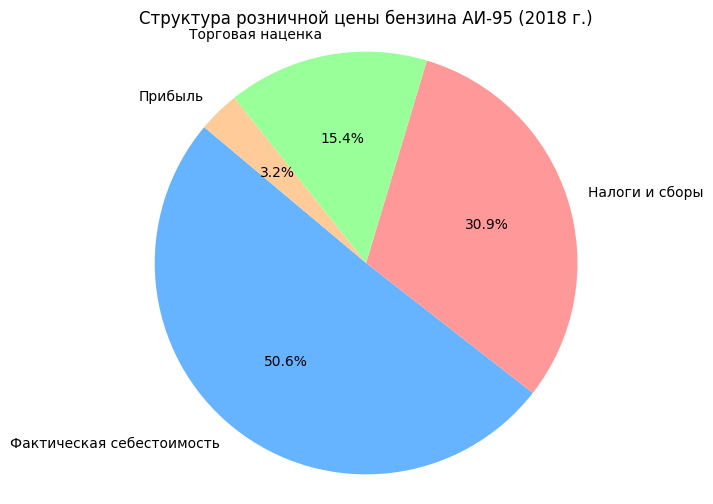
\includegraphics[scale=0.4]{graphs/5.4.png}

\end{document}